\newpage
%!TEX root = ../../main.tex
\section{Systemarkitektur}

I det følgende afsnit beskrives arkitekturen for systemet. Afsnittet fungerer som en vejledning og afgrænsning for udviklere på dette projekt. Hvis man vil videreudvikle på systemet er her et godt sted at starte med at få en grundlæggende idé om projektets opbygning. Her beskrives systemets moduler i forskellige former for diagrammer. På figur \ref{ArkiDia} kan man se en overordnet opbygning af systemet.

\begin{figure}[H]
	\centering
	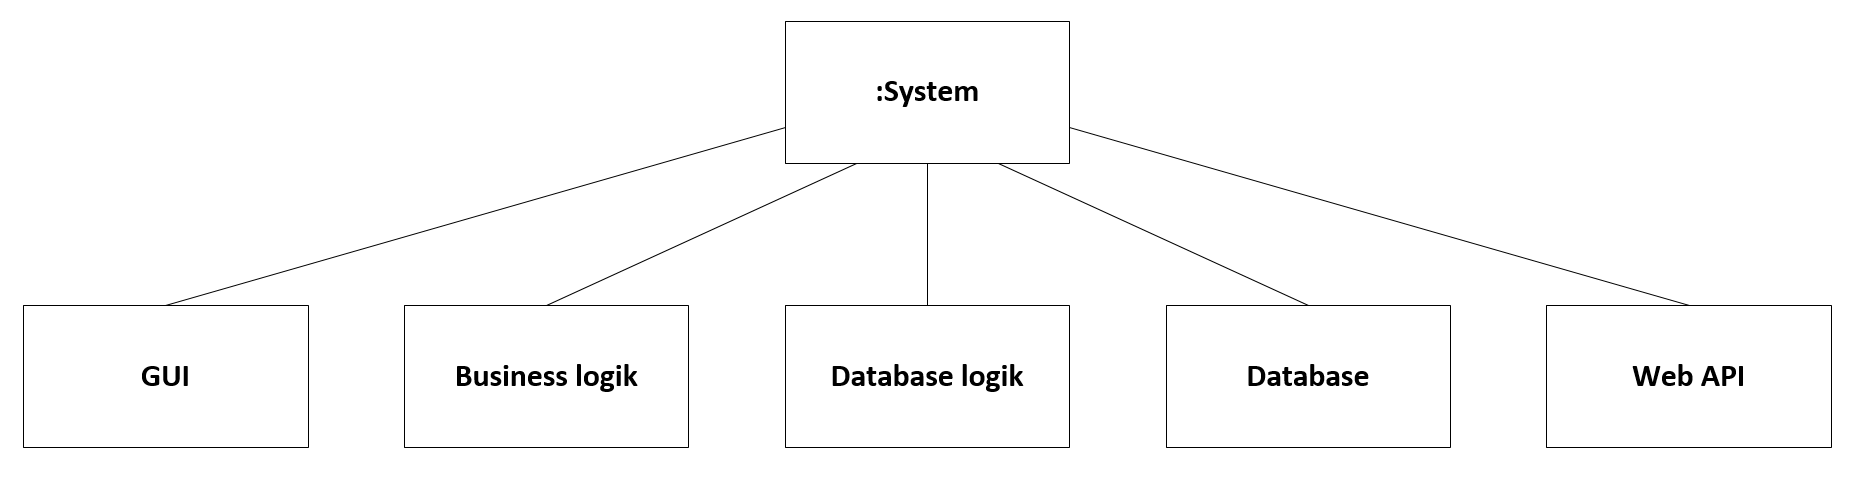
\includegraphics[scale=0.3]{Rapport/ArkitekturDiagram2}
	\caption{Overordnet arkitekturdiagram}
	\label{ArkiDia}
\end{figure}

\textbf{GUI} er ansvarlig for interaktion mellem Bartenderen og systemet. \gls{GUI}'en er det eneste som Bartenderen ser, han ved intet om systemets indre funktionalitet.
\newline\newline
\textbf{Business logikken} er al funktionaliteten i systemet. Her sker oprettelse af ordrer og transaktioner.
\newline\newline
\textbf{Databasen logikken} står for alt kommunikation med databasen. 
\newline\newline
\textbf{Database} indeholder alt information lige fra data om produkter og produktgrupper til ordrer og transaktioner.
\newline\newline
\textbf{Web API} bruges af web interfacet som er fronten til at oprette, redigere og fjerne produkter. Her kan der også ses statistik over salg. Det er denne som Administrator bruger til at tilgå systemet. 

\subsection{N+1 view}

\subsubsection{Use Case View}
I Use Case Viewet kan der ses hvordan de forskellige Use Cases beskriver systemet. Der er i dokumentationen indsat overordnede diagrammer der beskriver handlingsforløbet for hver af de fully dressed Use Cases.

\subsubsection{Logical View}
Logical View er en oversigt over hvordan programmet er bygget op. Logical View viser her hvordan det er valgt at dele systemet op i lag for at give mere overskuelighed. Her er der tale om:
\begin{itemize}
	\item Presentation Layer
	\item Business Layer
	\item Data Layer
	\item Web API
\end{itemize}
 
\textbf{Presentation Layer} indeholder alt omkring GUI og hvordan den er bygget op ved hjælp af MVVM. Her introduceres de forskellige views; SalesView, NumpadView, TabView, SettingsView. Disse bliver alle modelleret af en tilhørende Viewmodel således at de forskellige views intet kendskab har til Business Layer. \textbf{Business Layer} indeholder alt omkring oprettelse af ordrer og transaktioner. Dette lag kommunikerer med Presentation Layer og ligeledes med Data Layer. Det er Business Layer der sørger for at hente gemte data i Data Layer og ligeledes give data til Presentation Layer.\newline
\textbf{Data Layer} står for al persistering af data. Her bliver data gemt i en database og ligeledes hentet derfra. Data kan kun blive tilgået via \texttt{DAL}, Data Access Layer.\newline
\textbf{Web API} sørger for at det er muligt at oprette, redigere og fjerne produkter fra databasen. Her er det også muligt at få vist statistik over igangværende og forhenværende salg i systemet. 

\subsubsection{Domain View}
Domain View indeholder tankerne bag arkitekturen af systemet. Ud fra de definerede Use Cases blev der udtænkt nogle forskellige domæner der hver især har nogle ansvarsområder.\newline
De forskellige domæner i systemet er:\newline
\begin{itemize}
	\item IPaymentController
	\item IProductController
	\item IProductGroupController
	\item IDiscountController
	\item IReceiptController
	\item ILog, IPrinter
\end{itemize}	

\texttt{IPaymentController} har ansvar for de forskellige betalingsmetoder under en transaktion. \texttt{IProductController} har ansvar for de products der er i systemet, hvortil der kan oprettes, redigeres og fjernes. 
\texttt{IProductGroupController} har ansvar for at håndtere de forskellige Produkter i deres tilhørende produktgruppe.
\texttt{IDiscountController} har ansvar for at sørge for at den rigtige rabat bliver givet til de forskellige products.
\texttt{IReceiptController} har ansvar for at gemme de ordrer der er foretaget i løbet af en dag.
\texttt{ILog, IPrinter} er et specielt domæne der omhandler og har ansvar for at logge hændelser i systemet hvilket bliver skrevet til en fil. Her ligger ansvaret for at udskrive en kundebon også.


\subsubsection{Deployment View}
I Deployment View ses der hvordan systemet kunne udrulles og sættes op. Her er det vigtig at bide mærke i at selve databasen og \gls{WebAPI}'et kunne sættes op på deres egne seperate computere fungerende som server, og GUI'en og business logikken, kunne køre på en anden computer som så kunne kobles op til serveren. I vores system som det er udviklet, ligger databasen på samme computer som resten af systemet. \newline\newline
\begin{figure}[H]
	\centering
	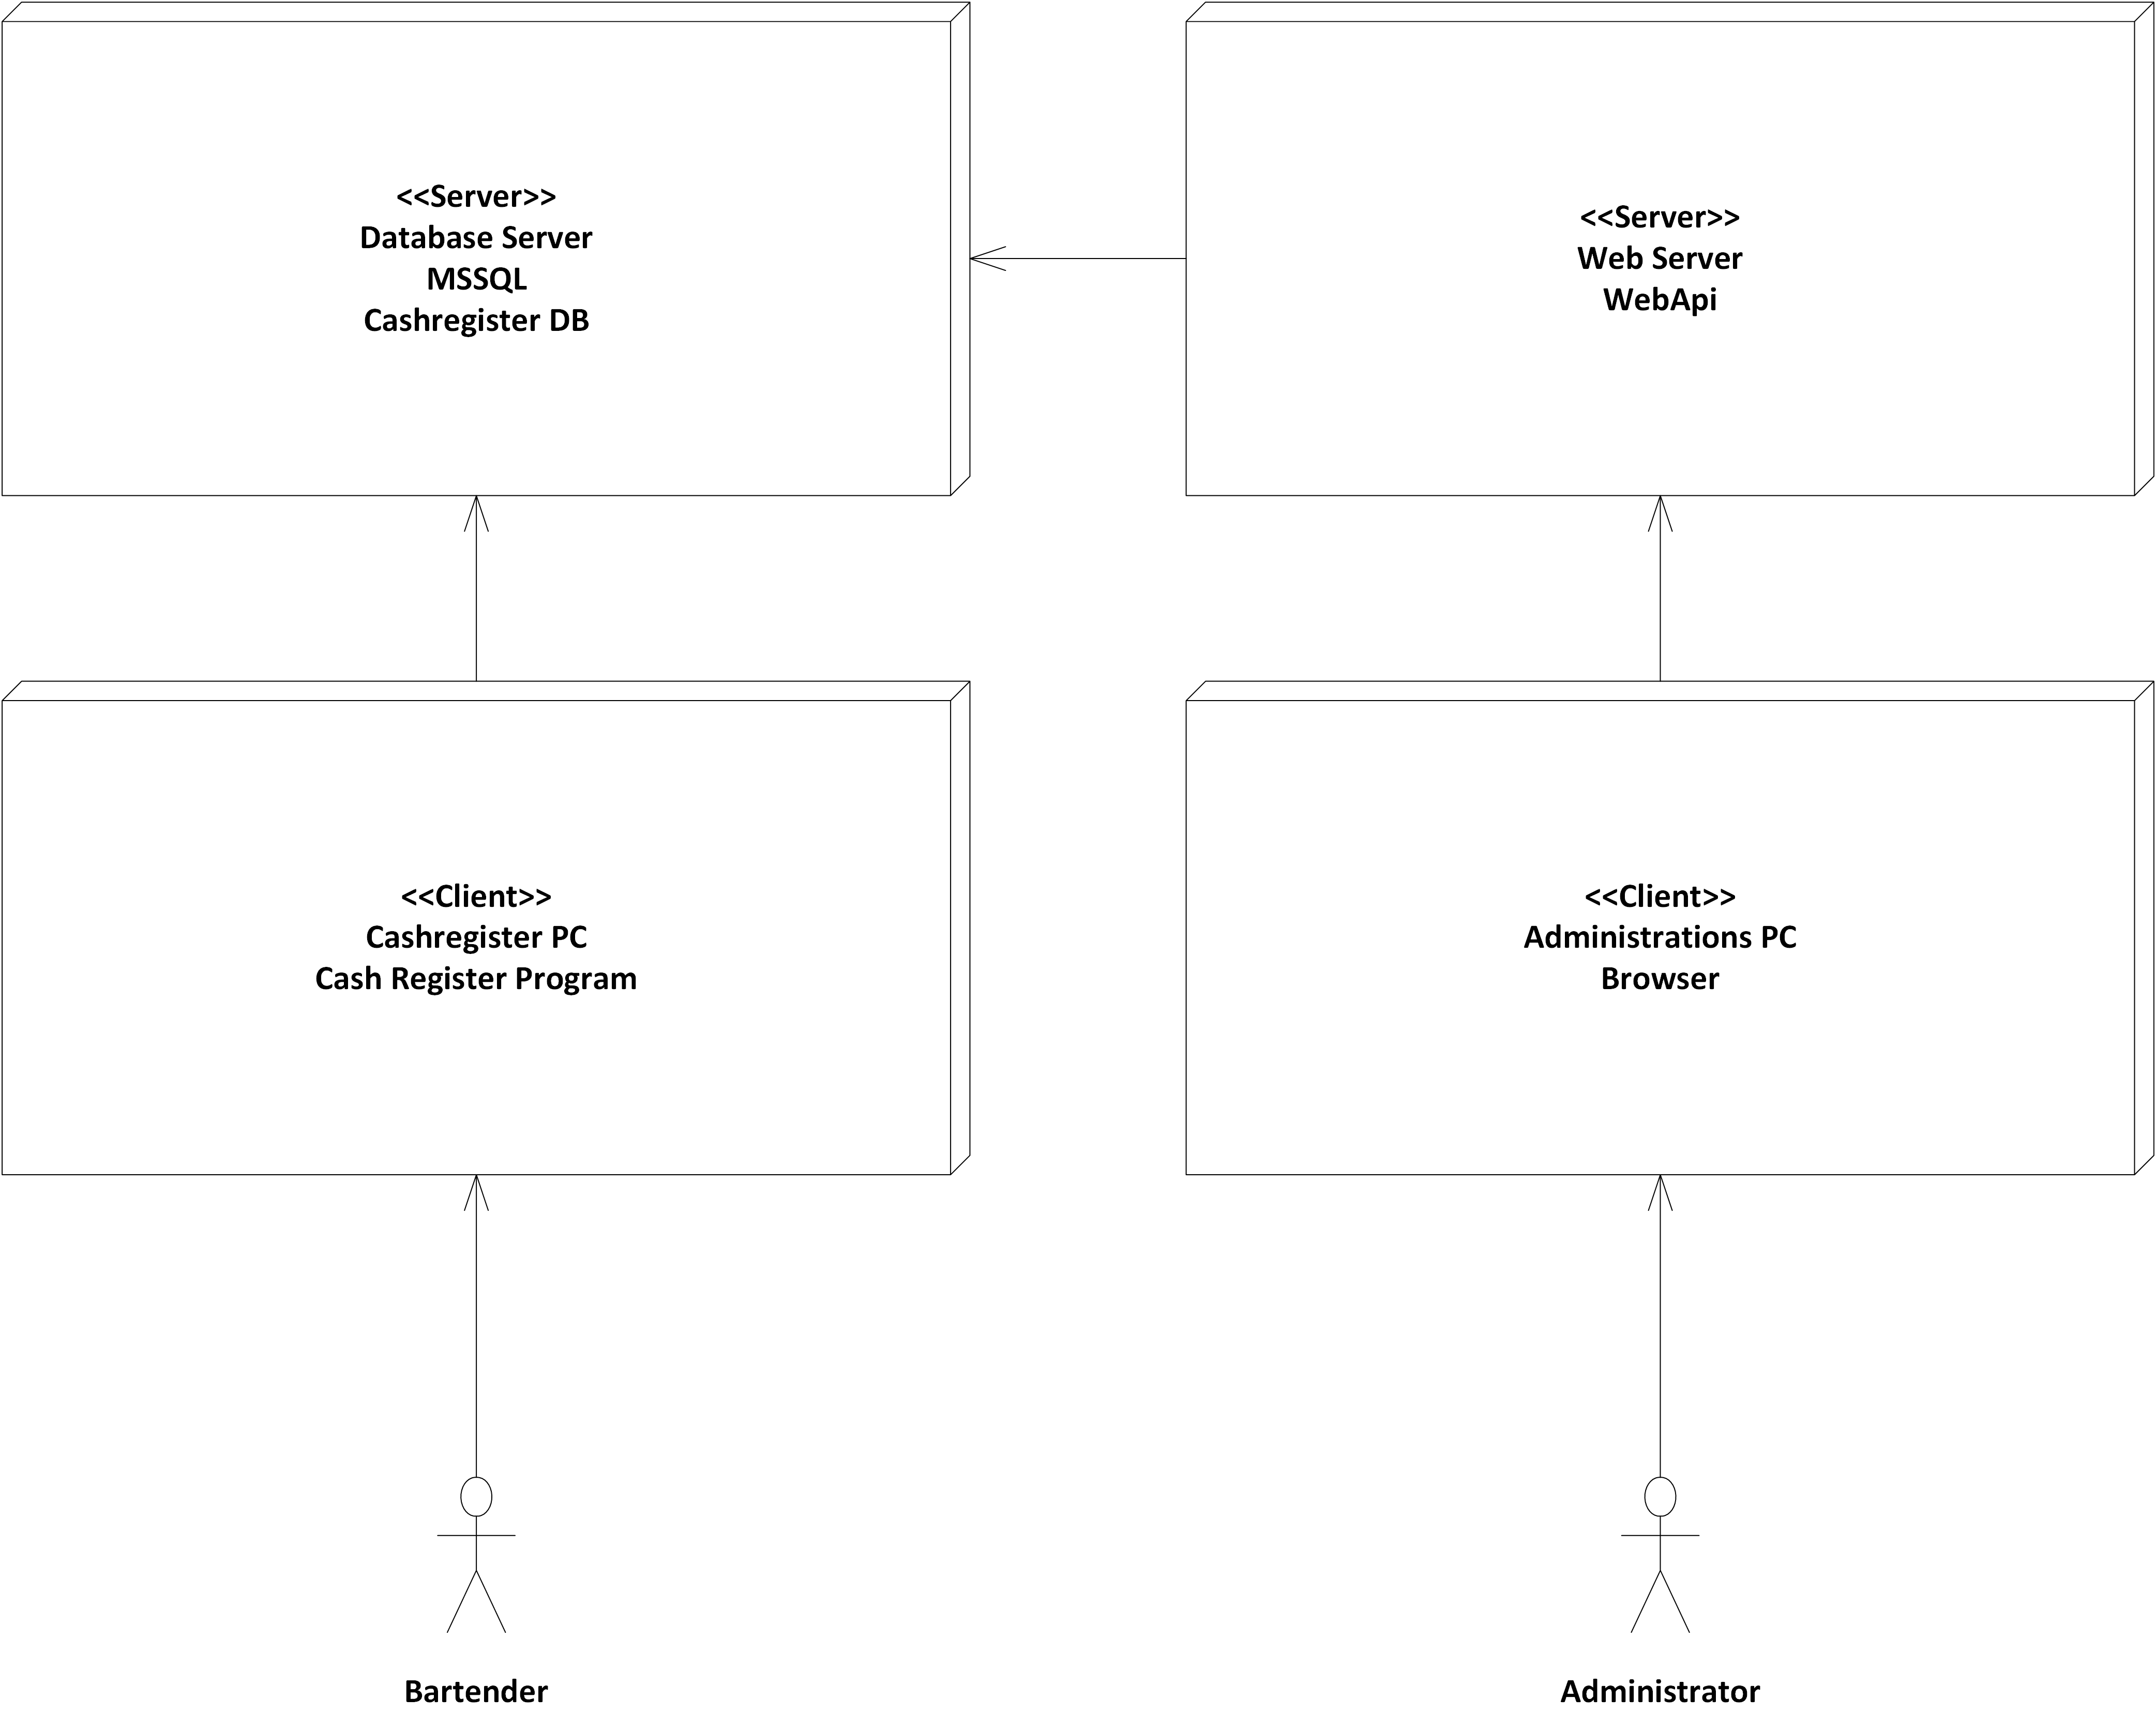
\includegraphics[scale=0.6]{/N+1/DeploymentView/System/Diagrammer/DEPLOY}
	\caption{Diagram over deployment af system}
	\label{fig:DeplayDia}
\end{figure}
Som det ses af figur \ref{fig:DeplayDia} kunne man sætte en administrations PC op som ville koble op til en Web Server som ville hoste Web API'et. Web API'et ville så tilkoble sig Database serveren so  ville køre på en seperat server. Hertil ville CashRegister programmet så køre på en seperat PC som bartenderen ville have adgang til. Dette betyder at man kunne opsætte flere kasseapparater som kunne koble op til samme database.  

\subsubsection{Data View}
I data view beskrives overgangen fra objekter i systemet til databasen. Her bliver der gennemgået Mapping til databasen sker.\newline\newline
I dokumentationen er der beskrevet hvor de forskellige klasser er blevet mappet til databasen. Her bliver der gennemgået hvorfor tabellerne er sat op som de er, og hvordan deres forhold til hinanden er. Her er klasse modeller og de fysiske modeller sat op over for hinanden så man hurtig kan se forskelle og ligheder.

\begin{figure}[H]
	\centering
	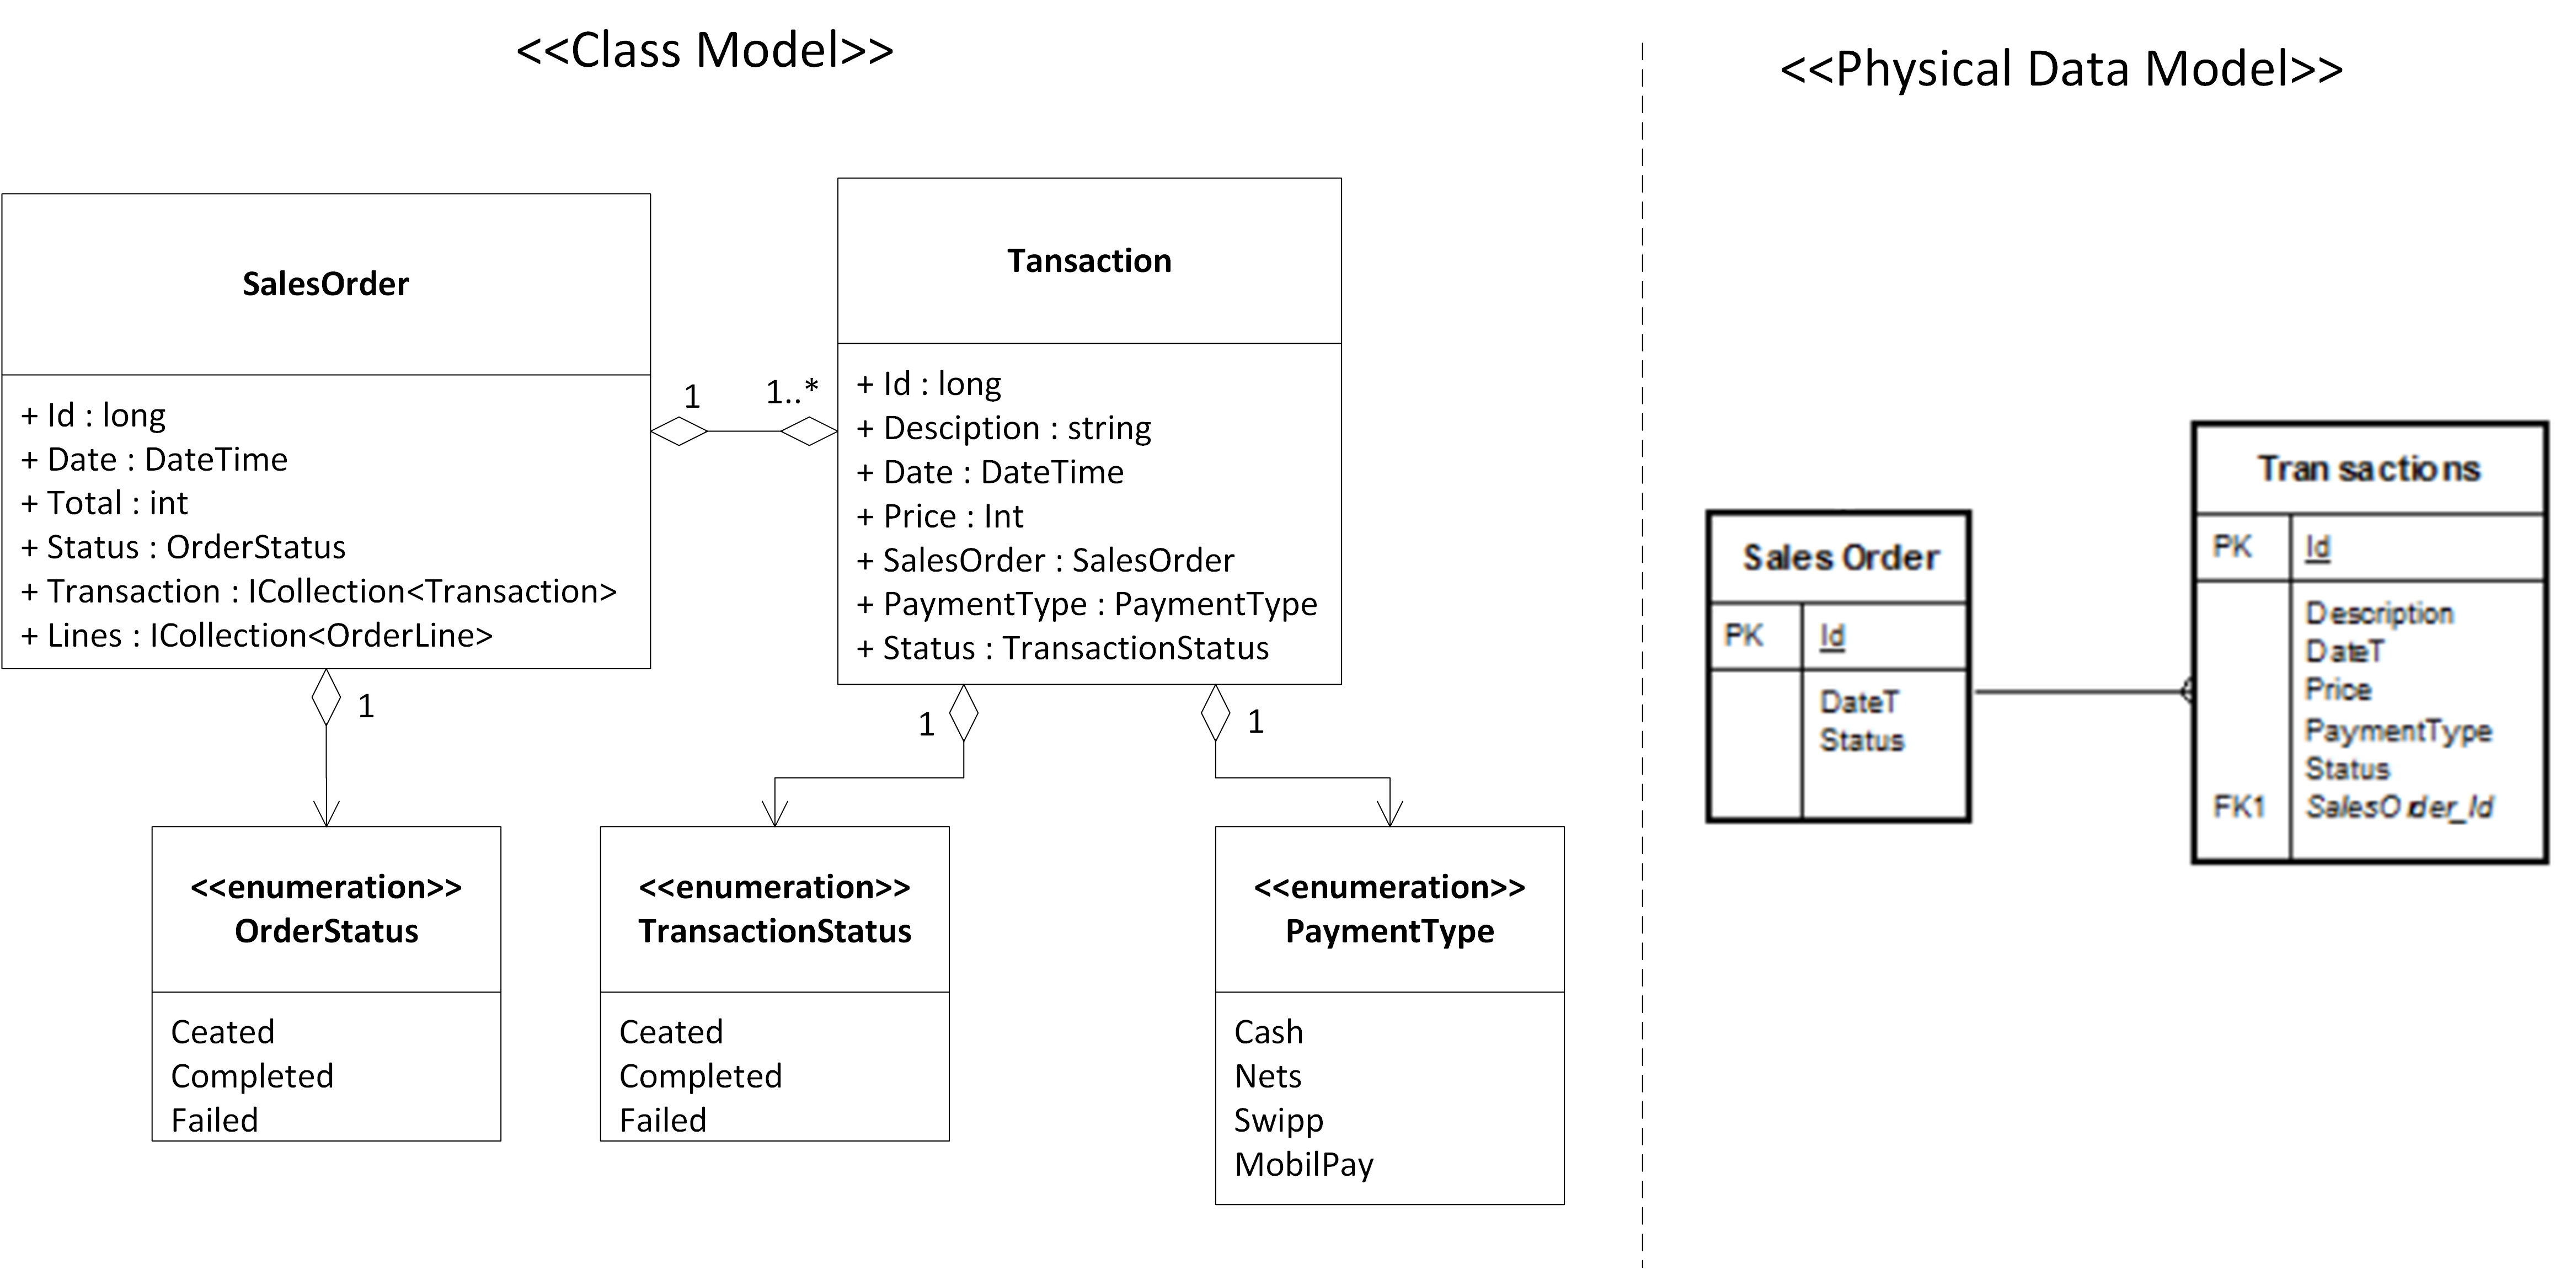
\includegraphics[scale=0.6]{/N+1/DataView/mapping/Mapping1}
	\caption{Diagram over objekt mapping}
	\label{MapDia}
\end{figure}	

På figur \ref{MapDia} ses det hvordan kobling af SalesOrder sker til Databasen. Her kan det ses at der mellem SalesOrder og Transaction er et one-to-many forhold og at Transaction har en fremmednøgle til SalesOrder.\newline\newline
Ydermere kan der i Data View ses hvordan dataflows sker fra én handling til den næste sker. Hertil er der lavet nogle aktivitetsdiagrammer ud fra de definerede Use Cases. 


\begin{figure}[H]
	\centering
	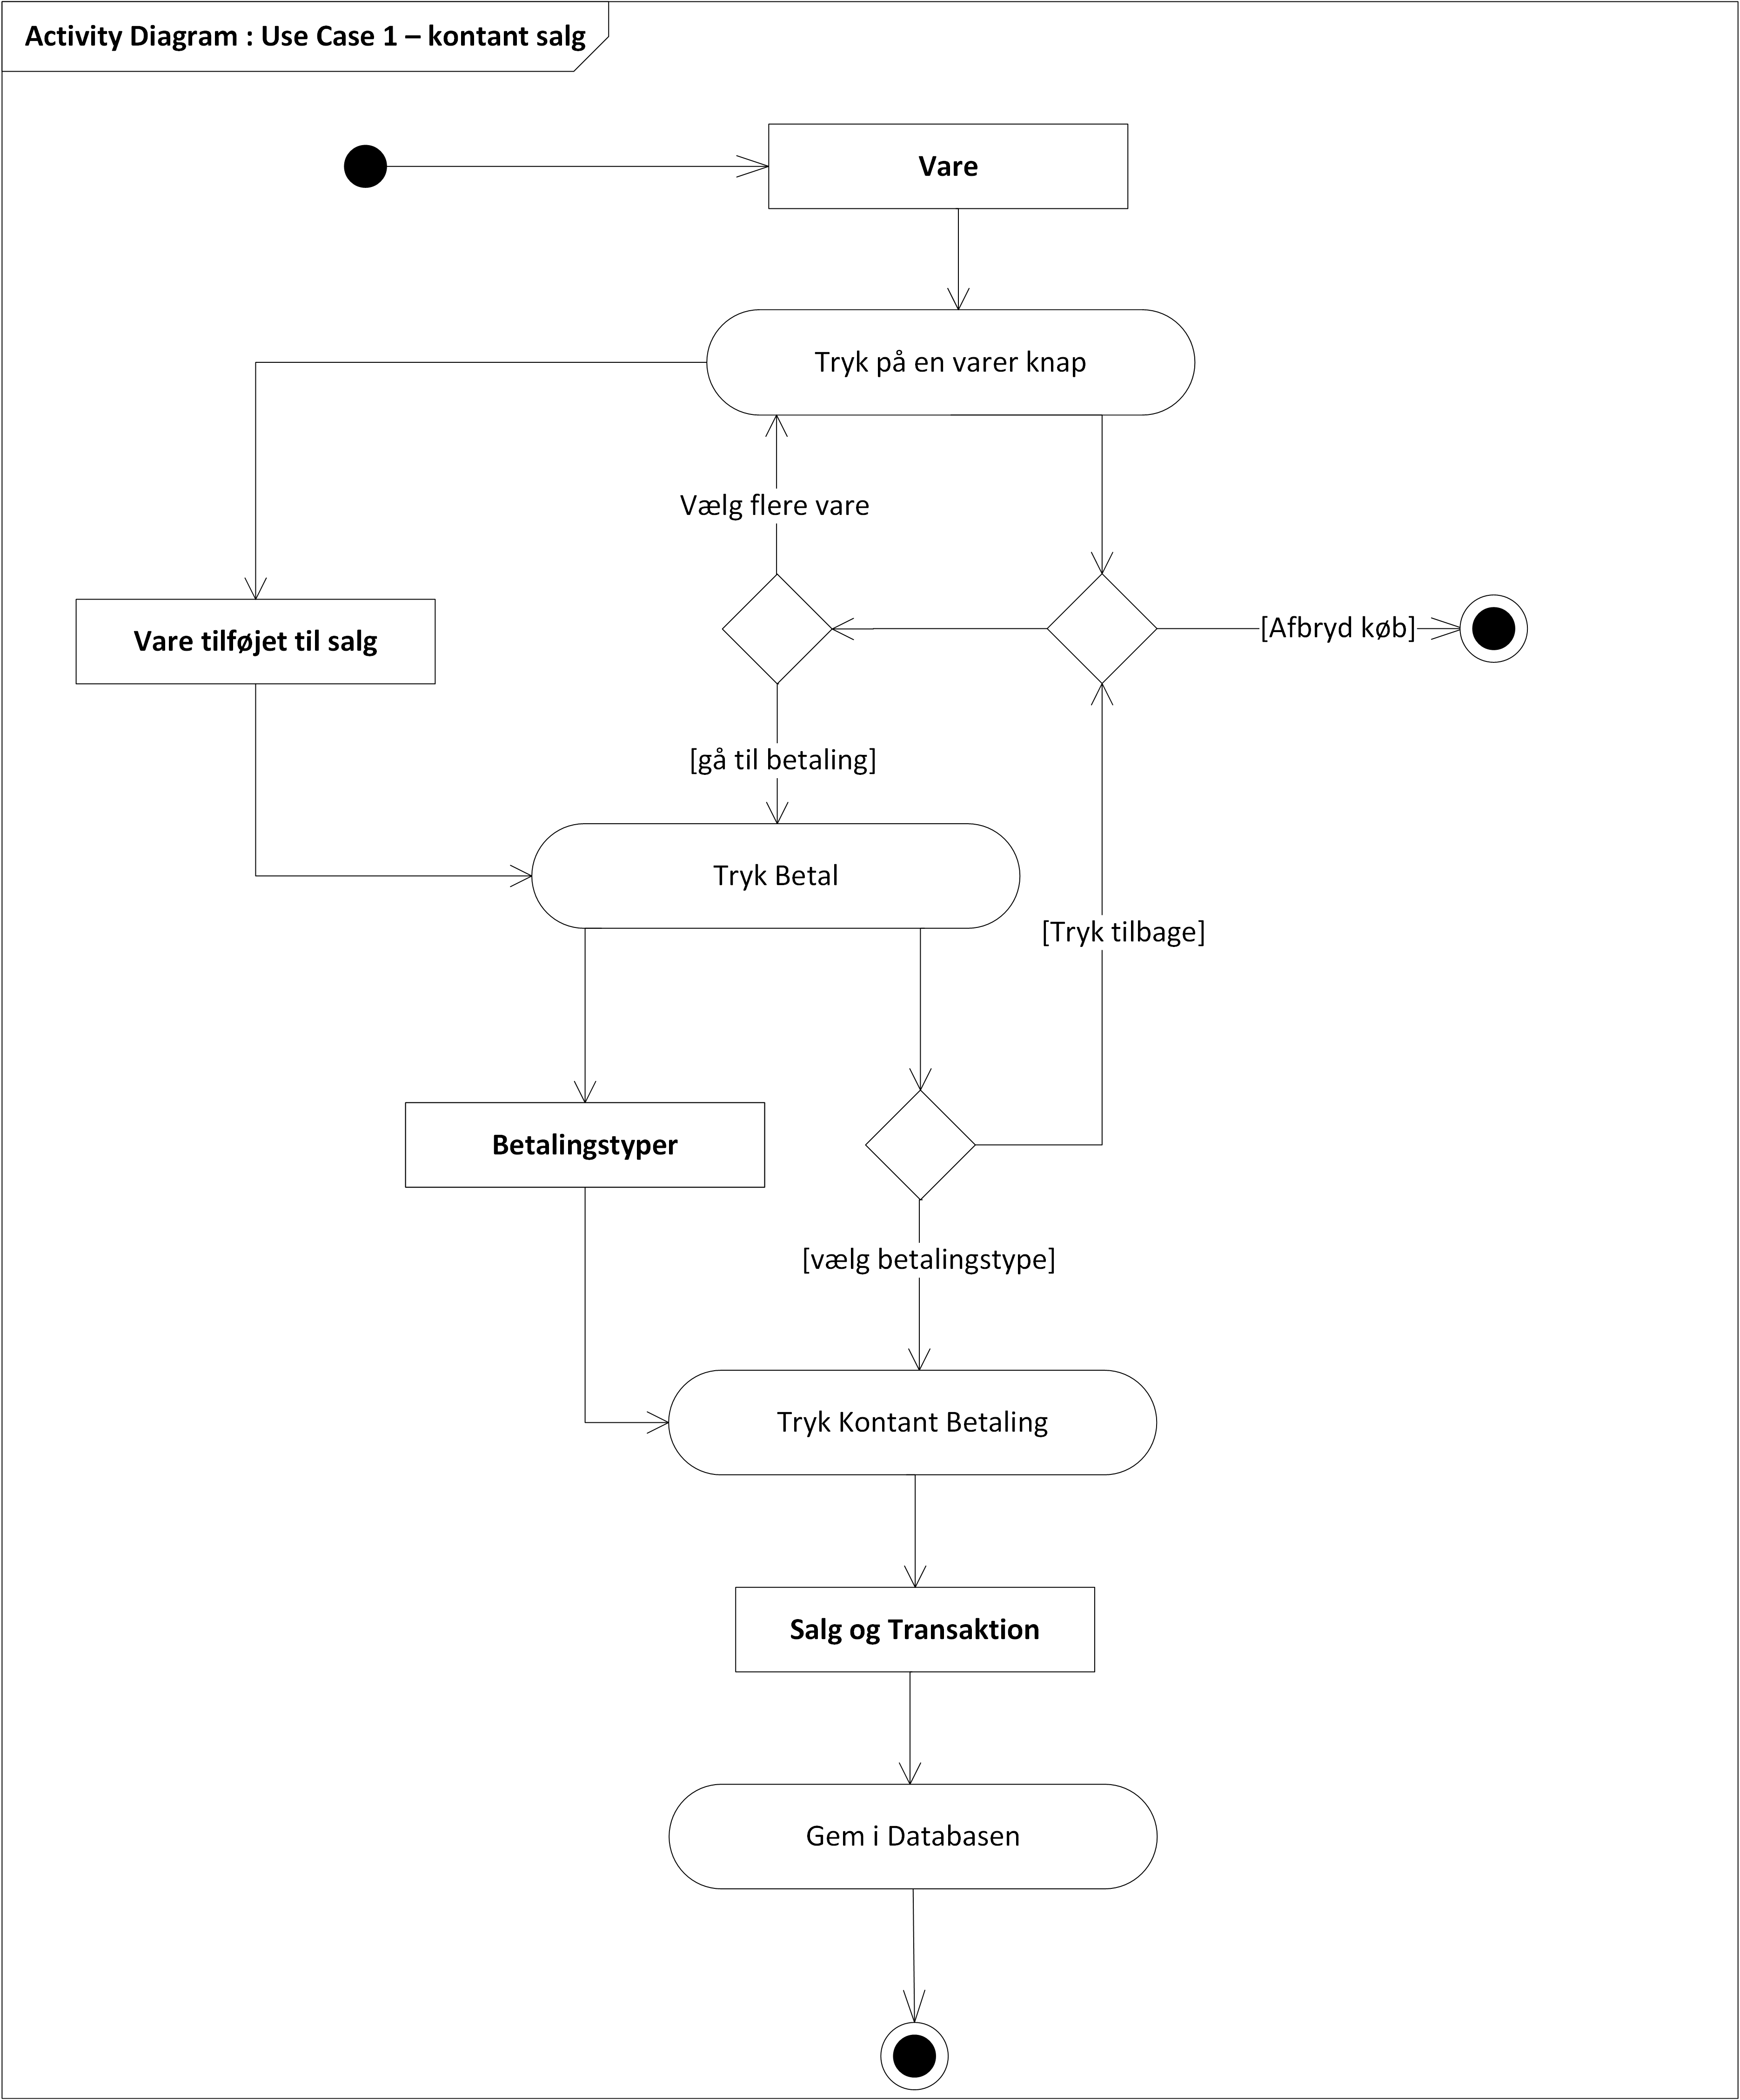
\includegraphics[scale=0.6]{/N+1/DataView/DataFlow/UC1}
	\caption{Aktivitetsdiagram over Use Case 1}	
	\label{AktDia}
\end{figure}

På figur \ref{AktDia} er dataflowet i forhold til Use Case 1 illustreret via et aktivitetsdiagram. Aktiviteterne gentages i nogle tilfælde og kører derfor i en løkke, og det kan også ses hvornår Use Casen og hvordan Use Casen afsluttes. Alt dette står mere detaljeret beskrevet i dokumentationen. 

 
 
  

